\documentclass{report}
\usepackage{graphicx, tikz-cd, float, titlepic, booktabs} % Required for inserting images
\usepackage{amsmath, amssymb, amsthm, amsfonts, siunitx, physics, gensymb}
\AtBeginDocument{\RenewCommandCopy\qty\SI}
\usepackage[version=4]{mhchem}
\usepackage[most,many,breakable]{tcolorbox}
\usepackage{xcolor, fancyhdr, varwidth}
\usepackage[Glenn]{fncychap}
%Options: Sonny, Lenny, Glenn, Conny, Rejne, Bjarne, Bjornstrup
\usepackage{hyperref, cleveref}
\usepackage{icomma, enumitem} %comma as decimal and continue enumerate with [resume]
\usepackage[danish]{babel}
%%%%%%%%%%%%%%%%%%%%%%%%%%%%%%
% SELF MADE COLORS
%%%%%%%%%%%%%%%%%%%%%%%%%%%%%%
\definecolor{myg}{RGB}{56, 140, 70}
\definecolor{myb}{RGB}{45, 111, 177}
\definecolor{myr}{RGB}{199, 68, 64}
\definecolor{mytheorembg}{HTML}{F2F2F9}
\definecolor{mytheoremfr}{HTML}{00007B}
\definecolor{mylenmabg}{HTML}{FFFAF8}
\definecolor{mylenmafr}{HTML}{983b0f}
\definecolor{mypropbg}{HTML}{f2fbfc}
\definecolor{mypropfr}{HTML}{191971}
\definecolor{myexamplebg}{HTML}{F2FBF8}
\definecolor{myexamplefr}{HTML}{88D6D1}
\definecolor{myexampleti}{HTML}{2A7F7F}
\definecolor{mydefinitbg}{HTML}{E5E5FF}
\definecolor{mydefinitfr}{HTML}{3F3FA3}
\definecolor{notesgreen}{RGB}{0,162,0}
\definecolor{myp}{RGB}{197, 92, 212}
\definecolor{mygr}{HTML}{2C3338}
\definecolor{myred}{RGB}{127,0,0}
\definecolor{myyellow}{RGB}{169,121,69}
\definecolor{myexercisebg}{HTML}{F2FBF8}
\definecolor{myexercisefg}{HTML}{88D6D1}
%%%%%%%%%%%%%%%%%%%%%%%%%%%%%%%%%%%%%%%%%%%%%%%%%%%%%%%%%%%%%%%%%%%%%%
% Box environments for theorems and problems
%%%%%%%%%%%%%%%%%%%%%%%%%%%%%%%%%%%%%%%%%%%%%%%%%%%%%%%%%%%%%%%%%%%%%
\setlength{\parindent}{1cm}
%================================
% Question BOX
%================================
\makeatletter
\newtcbtheorem{question}{Opgave}{enhanced,
	breakable,
	colback=white,
	colframe=myb!80!black,
	attach boxed title to top left={yshift*=-\tcboxedtitleheight},
	fonttitle=\bfseries,
	title={#2},
	boxed title size=title,
	boxed title style={%
			sharp corners,
			rounded corners=northwest,
			colback=tcbcolframe,
			boxrule=0pt,
		},
	underlay boxed title={%
			\path[fill=tcbcolframe] (title.south west)--(title.south east)
			to[out=0, in=180] ([xshift=5mm]title.east)--
			(title.center-|frame.east)
			[rounded corners=\kvtcb@arc] |-
			(frame.north) -| cycle;
		},
	#1
}{def}
\makeatother
%================================
% DEFINITION BOX
%================================

\newtcbtheorem[]{Definition}{Definition}{enhanced,
	before skip=2mm,after skip=2mm, colback=red!5,colframe=red!80!black,boxrule=0.5mm,
	attach boxed title to top left={xshift=1cm,yshift*=1mm-\tcboxedtitleheight}, varwidth boxed title*=-3cm,
	boxed title style={frame code={
					\path[fill=tcbcolback]
					([yshift=-1mm,xshift=-1mm]frame.north west)
					arc[start angle=0,end angle=180,radius=1mm]
					([yshift=-1mm,xshift=1mm]frame.north east)
					arc[start angle=180,end angle=0,radius=1mm];
					\path[left color=tcbcolback!60!black,right color=tcbcolback!60!black,
						middle color=tcbcolback!80!black]
					([xshift=-2mm]frame.north west) -- ([xshift=2mm]frame.north east)
					[rounded corners=1mm]-- ([xshift=1mm,yshift=-1mm]frame.north east)
					-- (frame.south east) -- (frame.south west)
					-- ([xshift=-1mm,yshift=-1mm]frame.north west)
					[sharp corners]-- cycle;
				},interior engine=empty,
		},
	fonttitle=\bfseries,
	title={#2},#1}{def}
\newtcbtheorem[]{definition}{Definition}{enhanced,
	before skip=2mm,after skip=2mm, colback=red!5,colframe=red!80!black,boxrule=0.5mm,
	attach boxed title to top left={xshift=1cm,yshift*=1mm-\tcboxedtitleheight}, varwidth boxed title*=-3cm,
	boxed title style={frame code={
					\path[fill=tcbcolback]
					([yshift=-1mm,xshift=-1mm]frame.north west)
					arc[start angle=0,end angle=180,radius=1mm]
					([yshift=-1mm,xshift=1mm]frame.north east)
					arc[start angle=180,end angle=0,radius=1mm];
					\path[left color=tcbcolback!60!black,right color=tcbcolback!60!black,
						middle color=tcbcolback!80!black]
					([xshift=-2mm]frame.north west) -- ([xshift=2mm]frame.north east)
					[rounded corners=1mm]-- ([xshift=1mm,yshift=-1mm]frame.north east)
					-- (frame.south east) -- (frame.south west)
					-- ([xshift=-1mm,yshift=-1mm]frame.north west)
					[sharp corners]-- cycle;
				},interior engine=empty,
		},
	fonttitle=\bfseries,
	title={#2},#1}{def}

\newtcbtheorem{theo}%
    {Theorem}{}{theorem}
\newtcolorbox{prob}[1]{colback=red!5!white,colframe=red!50!black,fonttitle=\bfseries,title={#1}}
%================================
% NOTE BOX
%================================

\usetikzlibrary{arrows,calc,shadows.blur}
\tcbuselibrary{skins}
\newtcolorbox{note}[1][]{%
	enhanced jigsaw,
	colback=gray!20!white,%
	colframe=gray!80!black,
	size=small,
	boxrule=1pt,
	title=\textbf{Note:},
	halign title=flush center,
	coltitle=black,
	breakable,
	drop shadow=black!50!white,
	attach boxed title to top left={xshift=1cm,yshift=-\tcboxedtitleheight/2,yshifttext=-\tcboxedtitleheight/2},
	minipage boxed title=1.5cm,
	boxed title style={%
			colback=white,
			size=fbox,
			boxrule=1pt,
			boxsep=2pt,
			underlay={%
					\coordinate (dotA) at ($(interior.west) + (-0.5pt,0)$);
					\coordinate (dotB) at ($(interior.east) + (0.5pt,0)$);
					\begin{scope}
						\clip (interior.north west) rectangle ([xshift=3ex]interior.east);
						\filldraw [white, blur shadow={shadow opacity=60, shadow yshift=-.75ex}, rounded corners=2pt] (interior.north west) rectangle (interior.south east);
					\end{scope}
					\begin{scope}[gray!80!black]
						\fill (dotA) circle (2pt);
						\fill (dotB) circle (2pt);
					\end{scope}
				},
		},
	#1,
}

%%%%%%%%%%%%%%%%%%%%%%%%%%%%%%%%%%%%%%%%%%%%%%%%%%%%%%%%%%%%%%%%%
% SELF MADE COMMANDS
%%%%%%%%%%%%%%%%%%%%%%%%%%%%%%
\newcommand{\sol}{\setlength{\parindent}{0cm}\textbf{\textit{Løsning:}}\setlength{\parindent}{1cm}}
%%%%%%%%%%%%%%%%%%%%%%%%%%%%%%%%%
\usepackage[tmargin=2cm,rmargin=1in,lmargin=1in,margin=0.85in,bmargin=2cm,footskip=.2in]{geometry}\pagestyle{fancy}
\lhead{Minrui Kevin Zhou 2.b}
\rhead{Matematikaflevering 15}

\title{Opgavesæt 3\\
{\Large \textbf{2.b kemi A}}}
\author{Kevin Zhou}
\date{Januar 2024}

\begin{document}
\maketitle
\section*{Opgave 1.15}
\sol \\
\textbf{a.} Afstemningen af reaktionsskemaet kan ses i \cref{fig:redox}.
\begin{figure}[H]
\begin{center}
  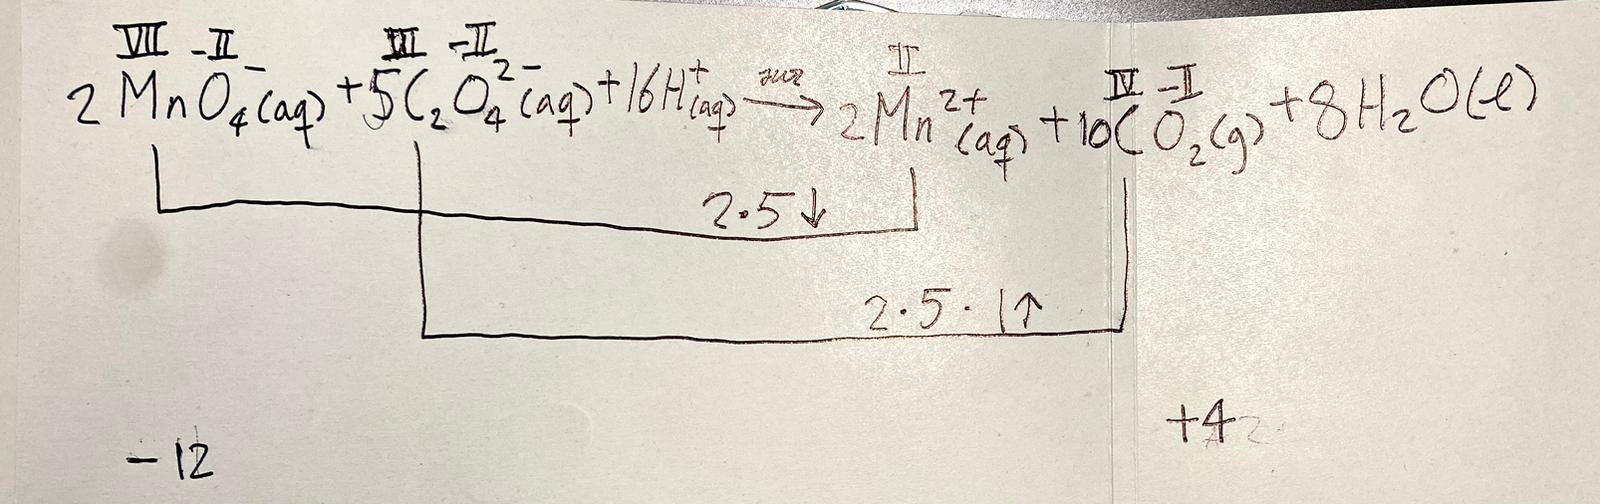
\includegraphics[width=\textwidth]{redox.jpeg}
\end{center}
\caption{Redoxreaktionen afstemt i hånden}
\label{fig:redox}
\end{figure}
\noindent \textbf{b.} 
Ved opløsningen af \ce{KMnO4} sker følgende reaktion.
\[
\ce{KMnO4(s) -> K+(aq) + MnO4-(aq)}
\] 
Altså er reaktionsforholdet mellem \ce{KMnO4} og \ce{MnO4-} 1:1.
Derfor gælder der, at
\[
[\ce{MnO4-}] = c(\ce{KMnO4})=0,02 \;\textsc{m}
\] 
\textbf{c.} Vi finder først stofmængden af \ce{MnO4-} og \ce{C2O4^2-}.
\[
n(\ce{MnO4-})=[\ce{MnO4-}]\cdot V=0,02 \;\unit{mol/L} \cdot 26,3 \;\unit{mL} = 0,526 \;\unit{mmol} 
\] 
Ved opløsning af \ce{Na2C2O4} er reaktionsforholdet mellem \ce{Na2C2O4} og \ce{MnO4-} 1:1.
Derfor gælder der, at
\[
n(\ce{C2O4^2-}) = n(\ce{Na2C2O4}) = m(\ce{Na2C2O4}) \cdot M(\ce{Na2C2O4})=\frac{0,189 \;\unit{g}}{134,00 \;\unit{g/mol} } = 1,4104\;\unit{mmol} 
\] 
Vi finder den begrænsende reaktant.
\begin{equation*}
\begin{split}
  n(\ce{MnO4-})\cdot 5 &=2,63 \;\unit{mmol} \\
  n(\ce{C2O4^2-}) \cdot 2 &\approx 2,821 \;\unit{mmol} 
\end{split}
\end{equation*}
Altså er \ce{MnO4-} den begrænsende reaktant og $n(\ce{CO2})=2,63 \;\unit{mmol} $.
Volumenet af \ce{CO2} dannet ved reaktionen kan nu regnes.
\[
V(\ce{CO2} )=24,4 \;\unit{L/mol} \cdot 2,63 \;\unit{mmol} \approx 64,2 \;\unit{mL}  
\] 
Man får dog ikke så meget \ce{CO2} som beregnet, da der altid vil gå lidt stof tabt ved eksempelvis skift af beholder.
Derudover opløses \ce{CO2}  i vandet i form af kulsyre.
\section*{Opgave 2.16}
\sol \\ 
\textbf{a.} 
Strukturformlerne for \textbf{X}, \textbf{Y} og \textbf{Z} ses i \cref{fig:xyz}.
\begin{figure}[H]
\begin{center}
  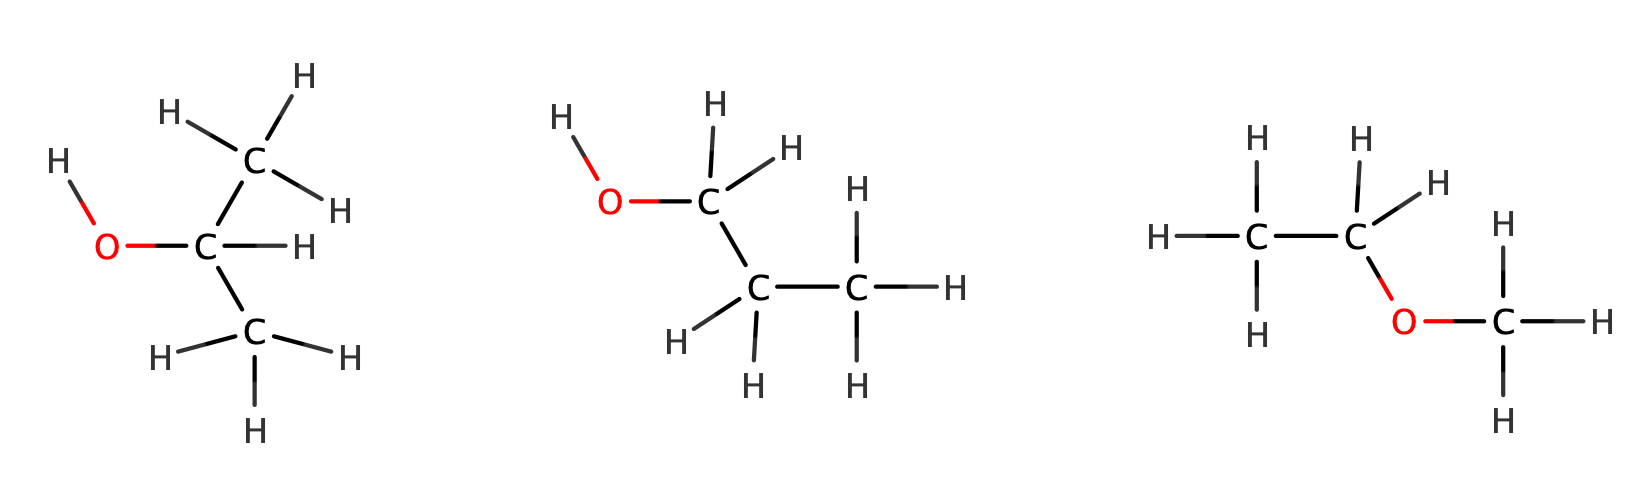
\includegraphics[width=\textwidth]{xyz.png}
\end{center}
\caption{Strukturformlerne for de tre stoffer tegnet i MarvinSketch}
\label{fig:xyz}
\end{figure}
\noindent\textbf{b.} 
Der er en polær elektronparbinding mellem \ce{C} og \ce{O}, siden $\Delta EN=1,0$.
Fra \cref{fig:xyz} får vi da så, at de første to molekyler er polære, hvor det tredje til højre ikke er.
Molekylet længst til højre må da have det laveste kogepunkt, da der så ikke er nogen dipol-dipolbindinger mellem molekylerne og må derfor være \textbf{X}.
Molekylet i midten er da mere aflangt mht. strukturformlen end molekylet længst til venstre og har da stærkere Londonbindinger.
Stukturformlen i midten må da være for \textbf{Z}.
Strukturformlen for \textbf{Y} er den til venstre.

Strukturformlerne i \cref{fig:xyz} er da respektivt for \textbf{Y, Z} og \textbf{X}. \\[1ex]
\noindent \textbf{c.} Et forslag på en strukturformel for \textbf{W} ses i \cref{fig:W}.
\begin{figure}[H]
\begin{center}
  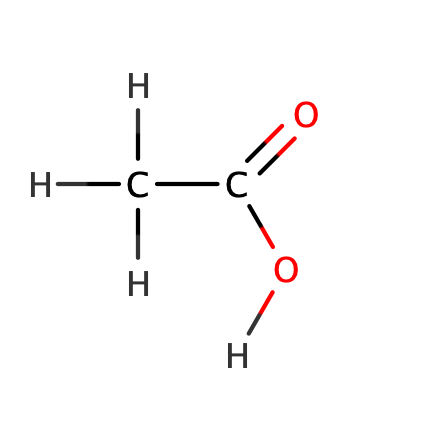
\includegraphics[scale=0.5]{W.png}
\end{center}
\caption{Forslag til strukturformel for \textbf{W} tegnet i MarvinSketch}
\label{fig:W}
\end{figure}
Det højere kogepunkt skyldes, at der udover dipol-dipolbindinger og Londonbindinger også forekommer hydrogenbindinger, der er stærkere end dipol-dipolbindinger.
Siden der er to oxygen-atomer, så kan den lave flere hydrogenbindinger.
\section*{Opgave 3.3}
\textbf{a.} Siden tetramminkobber(II) har en intens blå farve, så må der gælde, at absorptionsmaksimummet må ligge ved blås komplementærfarve, altså orange.
Det vil sige, at
\[
\lambda_{\text{max} }\approx 600 \;\unit{nm} 
\] 
\textbf{b.} Standardkurven ses i \cref{fig:Lambert}.
\begin{figure}[H]
\begin{center}
  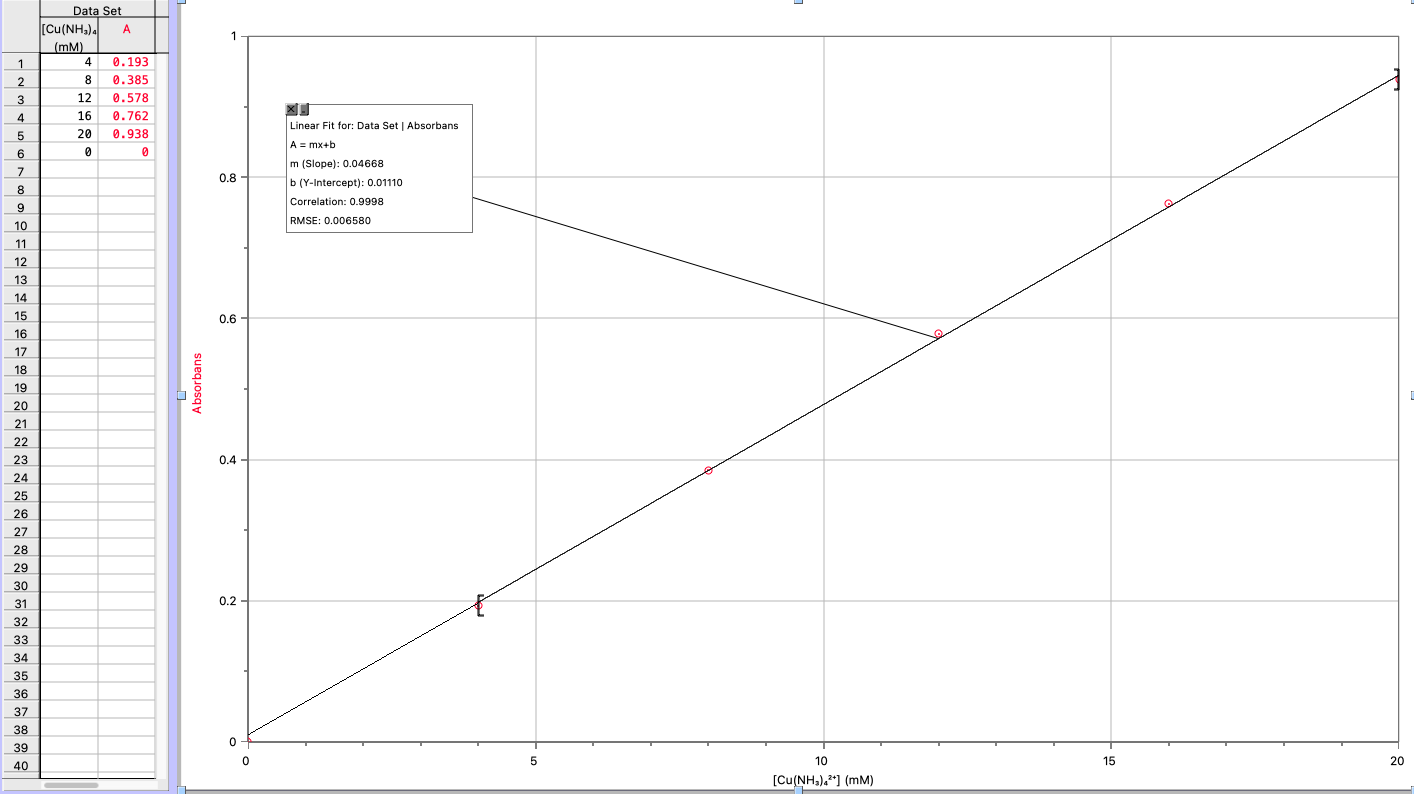
\includegraphics[width=\textwidth]{Lambert.png}
\end{center}
\caption{Standardkurven tegnet i Logger Pro}
\label{fig:Lambert}
\end{figure}
Siden målepunkterne tilnærmelsesvist ligger på en ret linje gennem (0,0), så understøtter det, at absorbansen er proportional med den aktuelle stofmængdekoncentration.
Altså følger resultaterne Lambert-Beers lov. \\[1ex]
\textbf{c.} Fra Lambert-Beers lov får vi, at 
\[
A=\varepsilon_\lambda \cdot l\cdot [S] \iff \frac{A}{[S]}=\varepsilon_\lambda \cdot l
\] 
Altså må hældningen på standardkurven svare til $\varepsilon_\lambda \cdot l$. 
Da lysvejen er $1,00 \;\unit{cm} $, så får vi
\[
\varepsilon_\lambda=\frac{0,04668}{ l\cdot \;\unit{m \textsc{m}}}=46,68 \;\unit{\textsc{m}^{-1}cm^{-1}} 
\] 
Ekstinktionskoefficienten er altså $46,68 \;\unit{\textsc{m}^{-1}cm^{-1}} $. \\[1ex]
\textbf{d.} 
Med vores model får vi, at den aktuelle stofmængdekoncentration af \ce{Cu(NH3)4^2+} er
\[
[\ce{Cu(NH3)4^2+}]=\frac{0,591-0.0111}{0,04668 \;\unit{m\textsc{m}^{-1}} }=12,42288 \;\unit{m\textsc{m}} 
\]
Fra følgende reaktionsskema får vi, at reaktionsforholdet mellem kobber(II)ionerne og tetramminkobber(II)ionerne er 1:1.
\[
\ce{Cu^2+ + 4NH3 -> Cu(NH3)4^2+} 
\] 
Vi får fra fortyndingsformlen, at koncentrationen af kobber(II)ioner i den mættede opløsning af kobber(II)sulfat er 100 gange større end koncentrationen af \ce{Cu(NH3)4^2+} i opløsning F.
\begin{equation*}
\begin{split}
  [\ce{Cu^2+} ]&=[\ce{Cu(NH3)4^2+}]\cdot \frac{V_{\text{efter} }}{V_{\text{før} }}\\ 
  &=12,42288 \;\unit{m\textsc{m}} \cdot \frac{100 \;\unit{mL} }{1,00 \;\unit{mL} }\\ 
  &=1,242288 \;\textsc{m} \approx 1,24 \;\textsc{m} 
\end{split}
\end{equation*}
Ved opløsningen af kobber(II)sulfatvand(1/5) i vand er reaktionsforholdet mellem \ce{CuSO4.5H2O} og \ce{Cu^2+} 1:1.
Altså må stofmængden og dermed koncentrationen være den samme.
Opløseligheden af kobber(II)sulfatvand(1/5) i vand må da være 
\[
c(\ce{CuSO4.5H2O})\cdot M(\ce{CuSO4.5H2O})=1,242288 \;\unit{mol/L} \cdot 249,69 \;\unit{g/mol} \approx 186 \;\unit{g/L} 
\] 
Altså får vi opløseligheden af kobber(II)sulfatvand(1/5) i vand til at være $186 \;\unit{g/L} $.
\end{document}
